\documentclass[12pt,a4paper]{article}
\usepackage[a4paper,left=1cm,right=1cm,top=2cm,bottom=2cm]{geometry}
\usepackage{xeCJK}
\setCJKmainfont[AutoFakeBold=true]{DFKai-SB}
\usepackage{tikz}
\usepackage{tikz-3dplot}
\usetikzlibrary{patterns,patterns.meta,arrows.meta,intersections,calc,decorations.pathmorphing}
\usepackage{pgfplots}
\usepackage{amsmath}
\usepackage{amssymb}
\usepackage{float}
\usepackage{cancel}
\usepackage{fancyhdr}
\usepackage{bm}
\usepackage{enumitem}
\usepackage{soul}
\pgfplotsset{compat=1.18}
\setlength{\headheight}{15pt}
\newcommand \dbar {{d\mkern-6mu\mathchar'26\mkern-3mu}}
\begin{document}

\setlist[enumerate,1]{label=\textbf{\alph*.}}
\setlist[enumerate,2]{label=\roman*.} % Fallback for deeper lists

% Custom problem list environment
\newlist{problems}{enumerate}{1}
\setlist[problems]{label={}, leftmargin=0pt, itemindent=0pt}

% Modified \problem command to include underline, dash, and percentage
\newcommand{\problem}[1]{%
  \item \underline{\textbf{Problem \arabic{problemsi} -- #1}}\par\vspace{0.2cm}
}

\begin{center}
    {\large \textbf{114-2 Separation Process (分離程序) Spring, 2026}}\\[0.3cm]
    {\Large \textbf{Homework\#3}}\\[0.3cm]
    {\textbf{Post: April 9\textsuperscript{th}, 2026; Due: April 23\textsuperscript{th}, 2026}}\\[0.4cm]
    \textbf{Name: 唐麒鈞 \quad Student ID: B10504001}
\end{center}
\vspace{0.8cm}
\begin{problems}
\problem{Example of ultrafiltration process}
The following two schematic illustrations display a single-stage and a two-stage ``feed and bleed'' ultrafiltration process.
The filtration area of the single-stage process is $A$,
and the filtration areas of the two-stage process are $A_1$ and $A_2$.\\
Use the \textbf{gel polarization model} to show that $A$ is always larger than ($A_1 + A_2$).\\
\textbf{Hint:} Consider using average flux and checking whether the gel polarization model is a concave or convex function.
\begin{figure}[H]
  \centering
  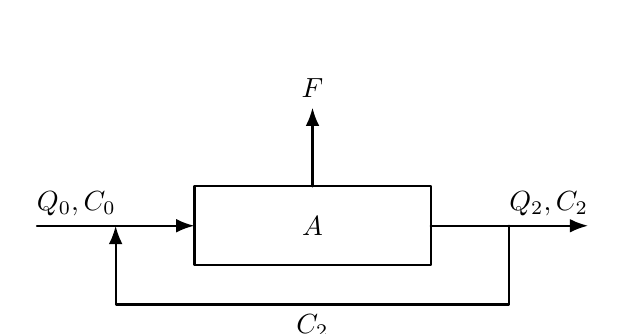
\begin{tikzpicture}[>=Latex, line cap=round, line join=round, thick]
    \draw[->] (0,0) -- (2,0);
    \node[anchor=south] at (0.5, 0) {$Q_0,C_0$};
    \draw (2,-0.5) rectangle (5,0.5);
    \node at (3.5, 0 ) {$A$};
    \draw[->] (3.5, 0.5) -- (3.5, 1.5) node[above] {$F$};
    \draw[->] (5,0) -- (7,0);
    \node[anchor=south] at (6.5, 0) {$Q_2,C_2$};
    \draw[->] (6,0) -- (6, -1) -- (1, -1) -- (1, 0);
    \node[anchor=north] at (3.5, -1) {$C_2$};
  \end{tikzpicture}
  \caption{Single `feed and bleed' stage}
\end{figure}
\begin{figure}[H]
  \centering
  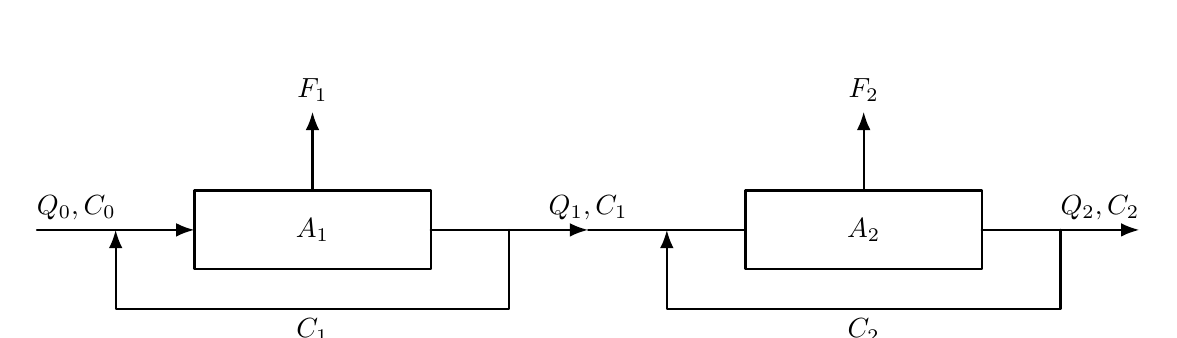
\begin{tikzpicture}[>=Latex, line cap=round, line join=round, thick]
    \draw[->] (0,0) -- (2,0);
    \node[anchor=south] at (0.5, 0) {$Q_0,C_0$};
    \draw (2,-0.5) rectangle (5,0.5);
    \node at (3.5, 0 ) {$A_1$};
    \draw[->] (3.5, 0.5) -- (3.5, 1.5) node[above] {$F_1$};
    \draw[->] (5,0) -- (7,0);
    \draw[->] (6,0) -- (6, -1) -- (1, -1) -- (1, 0);
    \node[anchor=north] at (3.5, -1) {$C_1$};
    \def\xShift{7}
    \draw (\xShift,0) -- (\xShift+2,0);
    \node[anchor=south] at (\xShift, 0) {$Q_1,C_1$};
    \draw (\xShift+2,-0.5) rectangle (\xShift+5,0.5);
    \node at (\xShift+3.5, 0 ) {$A_2$};
    \draw[->] (\xShift+3.5, 0.5) -- (\xShift+3.5, 1.5) node[above] {$F_2$};
    \draw[->] (\xShift+5,0) -- (\xShift+7,0);
    \node[anchor=south] at (\xShift+6.5, 0) {$Q_2,C_2$};
    \draw[->] (\xShift+6,0) -- (\xShift+6, -1) -- (\xShift+1, -1) -- (\xShift+1, 0);
    \node[anchor=north] at (\xShift+3.5, -1) {$C_2$};
  \end{tikzpicture}
  \caption{Two `feed and bleed' stages in series}
\end{figure}
\# Answer:\\
採用gel polarization model兩個設計假設：
\begin{enumerate}
  \item permeate concentration 幾乎為零，即 $C_p \approx 0$
  \item 在每一個 stage 中，flux expression 內的feed concentration 取該stage的retentate concentration
\end{enumerate}
Single-stage的flux expression\\
對任一stage，可寫成
\begin{equation}
  J(C)=h_D\ln\left(\frac{C_G}{C}\right)
\end{equation}
其中 $h_D$ 為mass-transfer coefficient，$C_G$ 為gel concentration\\
$C$為該stage 所對應的 retentate concentration。
對單一feed and bleed stage\\
solute balance
\begin{equation}
  Q_0C_0 = Q_2C_2
\end{equation}
overall fluid balance
\begin{equation}
  Q_0 = Q_2 + F
\end{equation}
所以
\begin{equation}
  F = Q_0 - Q_2
\end{equation}
single-stage的flux
\begin{equation}
  J_2 = h_D\ln\left(\frac{C_G}{C_2}\right)
\end{equation}
故所需膜面積為
\begin{equation}
  A = \frac{F}{J_2}
    = \frac{F}{h_D\ln\left(\dfrac{C_G}{C_2}\right)}
  \label{eq:A_single}
\end{equation}
Two-stage的flux expression\\
若改成兩段串聯，則由各段的 solute balance 可得
\begin{equation}
  Q_0C_0 = Q_1C_1 = Q_2C_2
\end{equation}
而fluid balance為
\begin{equation}
  F_1 = Q_0-Q_1,   \qquad F_2 = Q_1-Q_2
\end{equation}
因此總permeate flowrate為
\begin{equation}
  F = F_1 + F_2
  \label{eq:Fsum}
\end{equation}
同時兩段所需面積分別為
\begin{align}
  A_1 &= \frac{F_1}{J_1} = \frac{F_1}{h_D\ln\left(\dfrac{C_G}{C_1}\right)}\\
  A_2 &= \frac{F_2}{J_2} =  \frac{F_2}{h_D\ln\left(\dfrac{C_G}{C_2}\right)}
\end{align}
其中
\begin{equation}
  J_1 = h_D\ln\left(\frac{C_G}{C_1}\right),
  \quad
  J_2 = h_D\ln\left(\frac{C_G}{C_2}\right)
\end{equation}
因為兩段串聯時 $Q_0 > Q_1 > Q_2$，又有
\begin{equation}
  Q_0C_0 = Q_1C_1 = Q_2C_2
\end{equation}
所以
\begin{equation}
  C_0 < C_1 < C_2
\end{equation}
再考慮gel-polarization model的形狀：
\begin{equation}
  J(C)=h_D\ln\left(\frac{C_G}{C}\right)
\end{equation}
取微分
\begin{equation}
  \frac{dJ}{dC} = -\frac{h_D}{C} < 0
\end{equation}
再取微分
\begin{equation}
  \frac{d^2J}{dC^2} = \frac{h_D}{C^2} > 0
\end{equation}
因此$J(C)$對$C$是遞減且開口向上的函數\\
由於 $C_1 < C_2$，可知
\begin{equation}
  J_1 = J(C_1) > J(C_2)=J_2
  \label{eq:J1gtJ2}
\end{equation}
兩段串聯的總面積為
\begin{equation}
  A_1 + A_2 = \frac{F_1}{J_1} + \frac{F_2}{J_2}
  \label{eq:Atotal2}
\end{equation}
定義two-stage的average flux為
\begin{equation}
  \bar J_{\text{2-stage}} = \frac{F_1+F_2}{A_1+A_2}
  = \frac{F}{A_1+A_2}
\end{equation}
代入式\eqref{eq:Atotal2}可得
\begin{equation}
  \bar J_{\text{2-stage}}
  = \frac{F_1+F_2}{\dfrac{F_1}{J_1}+\dfrac{F_2}{J_2}}
\end{equation}
因為 $J_1>J_2$，所以
\begin{equation}
  J_2 < \bar J_{\text{2-stage}} < J_1
\end{equation}
同樣地，利用式\eqref{eq:Fsum}與\eqref{eq:A_single}，可得
\begin{equation}
  A_1+A_2
  = \frac{F}{\bar J_{\text{2-stage}}}
  < \frac{F}{J_2}
  = A
\end{equation}
故
\begin{equation}
  \boxed{A > A_1 + A_2}
\end{equation}
\problem{Conceptual questions}
\begin{enumerate}
\item Describe the \textbf{concentration polarization} and \textbf{gel-polarization model}.\\
Explain how concentration polarization occurs in ultrafiltration and identify two adverse effects of concentration polarization.\\
\# Answer:\\
Concentration polarization\\
在做Ultrafiltration的時候，溶劑穿過膜變成Permeate，而因為水一直往膜的方向流，就會把不能通過的溶質也更多的帶到膜的表面，導致膜表面的溶質濃度$C_w$超過原本液體的濃度$C_f$，造成Back-diffusion。\\
達到Steady state時
\begin{equation}
  J C_p = J C - \left(-D\frac{dC}{dy}\right)
\end{equation}
或者寫成
\begin{equation}
  J(C-C_p) = -D\frac{dC}{dy}
\end{equation}
其中$J$是permeate flux, $C_p$是透過趣的濃度, $D$是擴散係數。\\
如果把邊界層的厚度$l$考慮進去
\begin{equation}
  J = \frac{D}{l}\ln\left(\frac{C_w-C_p}{C_f-C_p}\right)
\end{equation}
假設溶質完全能被阻擋$C_p\approx 0$，可以簡化成
\begin{equation}
  J = \frac{D}{l}\ln\left(\frac{C_w}{C_f}\right)=h_D\ln\left(\frac{C_w}{C_f}\right)
\end{equation}
其中$h_D=D/l$是overall mass-transfer coefficient.\vspace{1cm}\\
Gel-polarization model\\
如果膜表面的溶質多到太誇張，就會卡在那裏變成像果凍一樣的Gel Layer。這時會有一個膜表面的極限濃度$C_G$
\begin{equation}
  J = h_D\ln\left(\frac{C_G}{C_f}\right)
\end{equation}
這個模型解釋了在Ultrafiltration 中，你以為增加壓力流速就會變快，但其實壓力變大，水流帶過去的溶質也變多，結果 Gel Layer 越長越厚，使得流速有一個極限值。\vspace{1cm}\\
identify two adverse effects of concentration polarization.
\begin{enumerate}
  \item 流速變慢
  \item 變得很難洗: Promotes Gel-layer/Cake-layer Formation
\end{enumerate}
\item Describe two membrane processes (\textbf{reverse osmosis}, \textbf{ultrafiltration}) used in liquid systems.
For each process, include the following: separation size range, driving force, and examples of separation applications.\\
\# Answer:
\begin{itemize}
  \item Reverse osmosis:
  \begin{itemize}
    \item Separation size range:\\
    能擋下極小的東西 $<1$ nm, 通常分子量 $<100$ Da
    \item Driving force：20 到 80 bar
    \item Typical applications:\\
    海水淡化、工業鍋爐給水、還有半導體在用的超純水製造
  \end{itemize}
  \item Ultrafiltration:
  \begin{itemize}
  \item Separation size range:\\
  colloids, proteins, macromolecules (about 1--100 nm, typically 1--500 kDa MWCO)
  \item Driving force: 1 到 10 bar
  \item Typical applicaion:\\
  濃縮蛋白質、Wastewater clarification，或是當作進去RO系統前的前處理，先幫RO擋下大顆粒免得它阻塞
  \end{itemize}
\end{itemize}
\item Describe the principles of \textbf{pervaporation} for liquid mixtures and explain how its separation mechanism differs from that of other membrane processes.\\
\# Answer:\\
Prevaporation就是一個進料端是液體，但在Permeate side故意抽真空或用惰性氣體吹，讓穿過去的成分直接變成氣體跑出來的方法。\\
另一邊很低的Partial pressure來當作推動力，而且用的是一層完全沒有孔的 Dense membrane。\\
而過濾的方式主要靠Solution–diffusion mechanism，可以拆成三個步驟：
\begin{enumerate}
\item Adsorption
\item Diffusion
\item Desorption
\end{enumerate}
最大的特色：有發生相變化，進去是液體，出來變氣體。\\
不是像一般過濾那樣單純把水擠過孔洞，而是先溶進去、再擴散、最後蒸發。\\
而且因為蒸發會吸熱，液體的溫度會下降\\
Pervaporation 跟其他膜製程差在哪？\\
膜長得不一樣：用的是完全沒有孔的Dense, nonporous selective layer\\
推動力不一樣：推動力是膜兩邊的Chemical potential、活性或 Partial pressure的差異\\
狀態不一樣：透過端會發生 Evaporation變成氣體
\item Describe the \textbf{membrane fouling}.\\
Explain how to prevent membrane fouling effects.\\
\# Answer:\\
Membrane fouling是指進料中的物質累積在膜表面或堵塞在膜孔中，導致膜性能，例如通量降低、選擇性變差之類的現象發生。\\
常見的foulants包括懸浮固體、膠體、有機物、微生物等。\\
而Fouling會造成清洗頻率上升、維護頻率上升、transmembrane pressure drop增加、membrane flux下降、selectivity改變、能耗上升等等。\\
Membrane fouling可分為以下幾種
\begin{itemize}
  \item Adsorption: 溶質吸附在膜表面或孔壁
  \item cake/gelation: 即顆粒或高分子在膜表面形成cake layer或gel layer
  \item pore blockage: 較大粒子或膠體堵住膜孔
\end{itemize}
若用膜過濾的一般式表示，fouling 會使 deposited layer resistance $R_c$增加，使得總阻力變大，導致通量下降
\begin{equation}
  J = \frac{\left|\Delta P\right|-\left|\Delta \pi\right|}{\mu(R_m + R_c)}
\end{equation}
How to prevent membrane fouling effects:
\begin{itemize}
  \item pretreatment of feed solution：\\
  先對進料做前處理，例如pre-filtration、調整 pH、控制 ionic strength\\
  以減少容易造成 fouling 的顆粒、膠體或聚集物
  \item change membrane properties：\\
  選擇較不易fouling的membrane material或表面性質，例如較親水、較平滑、抗吸附能力較好的膜。\\
  例如inorganic oxide membranes對fouling resistance 較佳。
  \item change process condition:\\
  改變操作條件來降低表面累積，\\
  例如提高 hydrodynamics、使用 cross-flow filtration 取代 dead-end filtration、採用 pulsed flow。\\
  P.S. cross-flow 可以把膜表面附近累積的 solute 帶走，因此能減少cake buildup與concentration polarization。
  \item cleaning:\\
  定期使用back flushing或chemical cleaning去移除已形成的foulant、cake或gel layer，恢復 membrane flux。
\end{itemize}
\end{enumerate}
\problem{Example of a Centrifugal separation}
A centrifuge basket, 750 mm long and 300 mm in internal diameter,
has a discharge weir with a diameter of 200 mm.\\
The retarding force on a particle moving in a liquid may be taken as $\bm{3\pi\mu du}$,
where $\bm{\mu}$ is the liquid viscosity, 
$\bm{d}$ is the particle diameter, and $\bm{u}$ is the particle velocity relative to the liquid.\\
The density of the liquid is 900 kg/m$^3$, the density of the solid is 2500 kg/m$^3$, and the viscosity
of the liquid is 1.1 cp (i.e., 0.0011 Pa$\cdot$s). 
The inertia of the particle may be neglected.
\begin{enumerate}
  \item What is the \textbf{maximum volumetric flow} of liquid through the centrifuge such that,
  when the basket is rotated at 300 Hz,
  all particles of diameter greater than 5 $\mu$m are retained on the centrifuge wall?
  \\
  \# Answer:\\
  先列出已知條件：
  \begin{align}
    H &= 0.75~\text{m} \\
    R &= \frac{0.300}{2} = 0.15~\text{m} \\
    r_o &= \frac{0.200}{2} = 0.10~\text{m} \\
    h &= R-r_o = 0.15-0.10 = 0.05~\text{m} \\
    \rho_l &= 900~\text{kg/m}^3 \\
    \rho_s &= 2500~\text{kg/m}^3 \\
    \Delta\rho &= \rho_s-\rho_l = 1600~\text{kg/m}^3 \\
    \mu &= 0.0011~\text{Pa}\cdot\text{s} \\
    d &= 5\times 10^{-6}~\text{m} \\
    \omega &= 2\pi N = 2\pi(300) = 1884.96~\text{rad/s}
  \end{align}
  $R$為centrifuge bowl radius，$r_o$為液面內半徑，$h$為液面厚度\\
  retarding force為$3\pi\mu d u$，所以對粒子來說
  \begin{equation}
    \frac{\pi}{6}d^3(\rho_s-\rho_l)r\omega^2 = 3\pi\mu d\,\frac{dr}{dt} \implies
    \frac{dr}{dt} = \frac{d^2(\rho_s-\rho_l)}{18\mu}\,r\omega^2
  \end{equation}
  retention time為
  \begin{equation}
    t_R = \frac{18\mu}{d^2(\rho_s-\rho_l)\omega^2}\ln\left(\frac{R}{r_o}\right)
  \end{equation}
  先檢查可否使用 $h\ll R$ 的近似：
  \begin{equation}
    \frac{h}{R} = \frac{0.05}{0.15} = \frac{1}{3}
  \end{equation}
  因此$h$沒有遠小於$R$，使用精確形式，centrifuge 內液體體積為
  \begin{equation}
    V' = \pi(R^2-r_o^2)H
  \end{equation}
  代入數值
  \begin{equation}
    V' = \pi(0.15^2-0.10^2)(0.75) = 2.945\times 10^{-2}~\text{m}^3
  \end{equation}
  對於 maximum throughput
  \begin{equation}
    \frac{V'}{Q_{\max}} = t_R
  \end{equation}
  也就是
  \begin{equation}
    Q_{\max} = \frac{V'}{t_R}
    = \frac{d^2(\rho_s-\rho_l)\omega^2V'}{18\mu\ln(R/r_o)}
  \end{equation}
  代入數值：
  \begin{equation}
    Q_{\max}
    = \frac{(5\times 10^{-6})^2(1600)(1884.96)^2(2.945\times 10^{-2})}{18(0.0011)\ln(0.15/0.10)}
    = 5.213518\times 10^{-1}~\text{m}^3/\text{s}
  \end{equation}
  換算為每小時流量：
  \begin{equation}
    Q_{\max} = 0.5213518\times 3600 = 1.87687\times 10^3~\text{m}^3/\text{h}
  \end{equation}
  答案為
  \begin{equation}
    \underline{Q_{\max} = 5.213518\times 10^{-1}~\text{m}^3/\text{s} \approx 1.1.87687\times 10^3~\text{m}^3/\text{h}}
  \end{equation}
  \item Discuss how the flow rate would change if the particle diameter decreased to 1 $\mu$m.
  \\
  \# Answer:\\
  由
  \begin{equation}
    Q_{\max} = \frac{d^2(\rho_s-\rho_l)\omega^2V'}{18\mu\ln(R/r_o)}
  \end{equation}
  可知在其他條件都固定時，
  \begin{equation}
    Q_{\max} \propto d^2
  \end{equation}
  因為粒徑由 $5~\mu\text{m}$ 降到 $1~\mu\text{m}$，所以最大可容許流量會變成原本的
  \begin{equation}
    \left(\frac{1}{5}\right)^2 = \frac{1}{25}
  \end{equation}
  因此
  \begin{equation}
    Q_{\max,\,1\mu\text{m}} = Q_{\max,\,5\mu\text{m}}\left(\frac{1}{5}\right)^2
    = \frac{0.521}{25}
    = 2.09\times 10^{-2}~\text{m}^3/\text{s}
  \end{equation}
  換算為每小時流量：
  \begin{equation}
    Q_{\max,\,1\mu\text{m}} = 2.09\times 10^{-2}\times 3600
    = 75.1~\text{m}^3/\text{h}
  \end{equation}
  \#從 $5~\mu\text{m}$ 降到 $1~\mu\text{m}$ 時，
  最大流量必須下降為原本的 $1/25$，也就是會變得更困難。
\end{enumerate}
\problem{Coulson \& Richardson's \textbf{Problem 8.1 (a)}}
Obtain expressions for the optimum concentration for minimum process time in the diafiltration of a solution of protein content $S$ in an initial volume $V_0$ if the gel-polarisation model applies.\\
It may be assumed that the extent of diafiltration is given by
\begin{equation}
V_d = \frac{\text{Volume of liquid permeated}}{\text{Initial feed volume}} = \frac{V_p}{V_0}
\end{equation}
\# Answer:\\
假設:
\begin{itemize}
  \item 膜會完全阻擋蛋白質
  \item 膜面積為$A$，且為constant
  \item Gel-polarization model
  \begin{equation}
    J = k \ln \left(\frac{C_g}{C}\right) \label{eq:gel_polarization}
  \end{equation}
  其中$k$為mass-transfer coefficient，$C_g$為gel concentration，$C$為Bulk concentration
\end{itemize}
總蛋白質質量守恆:
\begin{equation}
  C = \frac{S}{V},~ C_0 = \frac{S}{V_0} \implies V = \frac{S}{C}
\end{equation}
diafiltration前後的體積關係:
\begin{equation}
  \frac{dV}{dt} = -A J \implies dt = -\frac{dV}{AJ}  \label{eq:dt_dV}
\end{equation}
兩邊積分
\begin{equation}
  t_c = \int_0^{t_c} dt = -\int_{V_0}^{V} \frac{1}{Ak\ln\left(\frac{C_gV}{S}\right)}dV \label{eq:t_integral}
\end{equation}
假設$C_i$和$C_f$分別為diafiltration前後的蛋白質濃度，則
\begin{equation}
  \frac{C_f}{C_i} = \text{exp}\left(-\frac{V_p}{V}\right) \implies \frac{V_p}{V} = \ln\left(\frac{C_i}{C_f}\right)
\end{equation}
代入\eqref{eq:gel_polarization}到\eqref{eq:dt_dV}，得到diafiltration的時間
\begin{equation}
 t_d = \frac{V_p}{AJ} = \frac{V \ln\left(\frac{C_i}{C_f}\right)}{Ak \ln\left(\frac{C_g}{C}\right)} = 
 \frac{S \ln\left(\frac{C_i}{C_f}\right)}{Ak C \ln\left(\frac{C_g}{C}\right)} \label{eq:t_diafiltration}
\end{equation}
總時間為\eqref{eq:t_integral}與\eqref{eq:t_diafiltration}相加:
\begin{align}
  t &= t_c + t_d \nonumber\\
  &=- \left[\int_{V_0}^{V} \frac{1}{Ak\ln\left(\frac{C_gV}{S}\right)}dV\right] 
  + \frac{S \ln\left(\frac{C_i}{C_f}\right)}{Ak C \ln\left(\frac{C_g}{C}\right)} \label{eq:t_total}
\end{align}
定義$L$和$N$為:
\begin{equation}
  N \equiv \ln\left(\frac{C_i}{C_f}\right),\quad
  L \equiv \ln\left(\frac{C_g}{C}\right) = \ln\left(\frac{C_gV}{S}\right)
\end{equation}
因此
\begin{equation}
  \frac{dL}{dV} = \frac{1}{V}
\end{equation}
代入\eqref{eq:t_total}
\begin{equation}
  t = \frac{1}{Ak} \left[
    \int_V^{V_0} \frac{1}{L}dV + \frac{VN}{L}
  \right]
\end{equation}
對$V$微分，並取0為最佳解
\begin{equation}
  \frac{dt}{dV}  = 0 = \frac{1}{Ak}\left[
    -\frac{1}{L} + N \left(
      \frac{1}{L} - \frac{1}{L^2}
    \right)
  \right]
\end{equation}
化簡
\begin{align}
  &0 = -\frac{1}{L} + N \left(
    \frac{1}{L} - \frac{1}{L^2}
  \right) \nonumber\\
  \implies& -L + N(L-1) = 0 \nonumber\\
  \implies& (N-1)L = N \nonumber\\
  \implies& L = \frac{N}{N-1} \label{eq:L_optimal}
\end{align}
代回$L$和$N$的定義
\begin{equation}
  \ln\left(\frac{C_g}{C_{\text{opt}}}\right) = \frac{\ln\left(\frac{C_i}{C_f}\right)}{\ln\left(\frac{C_i}{C_f}\right)-1}
\end{equation}
因此得到最佳濃度$C_{\text{opt}}$
\begin{equation}
  \underline{C_{\text{opt}} = C_g \exp\left(-\frac{\ln\left(\frac{C_i}{C_f}\right)}{\ln\left(\frac{C_i}{C_f}\right)-1}\right)}
\end{equation}
\problem{Coulson \& Richardson's \textbf{Problem 9.3}}
A centrifuge basket 600 mm long and 100 mm internal diameter has a discharge weir 25 mm diameter.\\
What is the maximum volumetric flow of liquid through the centrifuge such that when the basket is rotated at 200 Hz all particles of diameter greater than 1 $\mu$m are retained on the centrifuge wall?\\
The retarding force on a particle moving liquid may be taken as $3\pi\mu du$,
where $u$ is the particle velocity relative to the liquid $\mu$ is the liquid viscosity,
and $d$ is the particle diameter.\\
The density of the liquid is 1000 kg/m$^3$,
the density of the solid is 2000 kg/m$^3$ and the viscosity of the liquid is 1.0 mN s/m$^2$.\\
The inertia of the particle may be neglected.\\
\# Answer:\\
先列出已知條件：
\begin{itemize}
  \item Basket length $L$ = 600 mm = 0.6 m
  \item Basket internal diamete $R_2$ = 100 mm / 2 = 0.05 m
  \item Weir radius $R_1$ = 25 mm / 2 = 0.0125 m
  \item Rotational speed $N$ = 200 Hz
  \item Angular velocity $\omega$ = $2\pi N$ = $2\pi \times 200$ = $400\pi$ rad/s
  \item Partical cut diameter $d$ = 1 $\mu$m = $1 \times 10^{-6}$ m
  \item Solid density $\rho_s$ = 2000 kg/m$^3$
  \item Liquid density $\rho_l$ = 1000 kg/m$^3$
  \item Viscosity $\mu$ = 1.0 mN s/m$^2$ = $1.0 \times 10^{-3}$ kg/(m$\cdot$s)
\end{itemize}
離心力$F_c$:
\begin{equation}
  F_c = m r\omega^2  = \frac{\pi}{6} d^3 (\rho_s - \rho_l)  r\omega^2
\end{equation}
Drag force $F_d$:
\begin{equation}
  F_d = 3\pi \mu d u_r,~\quad u_r = \frac{dr}{dt}
\end{equation}
忽略粒子慣性，則$F_c = F_d$，所以
\begin{equation}
  \frac{\pi}{6} d^3 (\rho_s - \rho_l)  r\omega^2 = 3\pi \mu d \frac{dr}{dt}
\end{equation}
得到$\frac{dr}{dt}$
\begin{equation}
  \frac{dr}{dt} = \frac{d^2 (\rho_s - \rho_l) r\omega^2}{18 \mu}
\end{equation}
積分上下界分別為$R_1$和$R_2$，得到retention time $t_R$
\begin{equation}
  \int_{R_1}^{R_2} \frac{dr}{r} = \int_0^{t_R} \frac{d^2 (\rho_s - \rho_l) \omega^2}{18 \mu} dt
\end{equation}
積分:
\begin{equation}
  \ln \left(\frac{R_2}{R_1}\right) = \frac{d^2 (\rho_s - \rho_l) \omega^2}{18 \mu} t_R \label{eq:lnR2R1}
\end{equation}
假設Plug flow, 軸向流速為$u_z$是uniform的，則可以得到$Q$
\begin{equation}
t_R = \frac{V}{Q} = \frac{\pi (R_2^2 - R_1^2) L}{Q}
\end{equation}
將$t_R$代入\eqref{eq:lnR2R1}，得到$Q$
\begin{align}
  \ln \left(\frac{R_2}{R_1}\right) &= \frac{d^2 (\rho_s - \rho_l) \omega^2}{18 \mu}\cdot \frac{\pi (R_2^2 - R_1^2) L}{Q}\\
  Q &= \frac{d^2(\rho_s - \rho_l) \omega^2}{18 \mu}\cdot \pi (R_2^2 - R_1^2) L \cdot \frac{1}{\ln\left(\frac{R_2}{R_1}\right)}
\end{align}
代入數值：
\begin{align}
  d^2(\rho_s - \rho_l) &= (1\times 10^{-6})^2 \times (2000 - 1000) = 1 \times 10^{-9}~\text{kg/m} \\
  \omega^2 &= (400\pi)^2 = 1.6 \times 10^5 \pi^2~\text{rad}^2/\text{s}^2 \\
  R_2^2 - R_1^2 &= 0.05^2 - 0.0125^2 = 0.00234375~\text{m}^2 \\
  \ln\left(\frac{R_2}{R_1}\right) &= \ln\left(\frac{0.05}{0.0125}\right) = \ln(4)
\end{align}
因此$Q$為
\begin{align}
  Q &= \frac{(1 \times 10^{-9})(1.6 \times 10^5 \pi^2)(\pi)(0.00234375)(0.6)}{18 (1.0 \times 10^{-3}) \ln(4)}\nonumber\\
  & =  2.79578 \times 10^{-4}~\text{m}^3/\text{s} 
\end{align}
答:
\begin{equation}
  \underline{Q_{\max} = 2.79578 \times 10^{-4}~\text{m}^3/\text{s}}
\end{equation}
\end{problems}
\end{document}
